\documentclass{article}
\usepackage[utf8]{inputenc}
\usepackage[russian]{babel}
\usepackage{graphicx}
\usepackage{csquotes}
\usepackage{pgf,tikz}
\usepackage{adjustbox}
\usepackage{mathrsfs}
\usepackage{amsmath}
\usetikzlibrary{arrows}
\pagestyle{empty}

\graphicspath{ {/home/denis/workspace/University/masters/machine-learning-agre/exercises/ex2/images/} }

\begin{document}
\title{Упражнение 2}
\author{Денис Симеонов Михайлов \\ ФН: 25788}
\date{28 октомври 2017г.}
\maketitle
\paragraph{1)}
Нарисувайте класификационни дървета, представящи следните Булеви функции:
\begin{enumerate}
\item [a)]$A \land \neg B$
	\begin{minipage}[t]{\linewidth}
          \raggedright
          \adjustbox{valign=t}{
            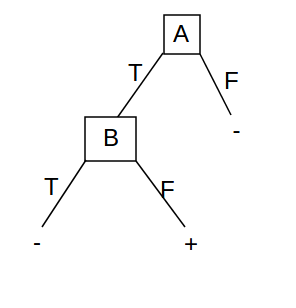
\includegraphics[width=.4\linewidth]{1a}
          }
    \end{minipage}
\item [b)]$A \lor [B \land C]$
	\begin{minipage}[t]{\linewidth}
          \raggedright
          \adjustbox{valign=t}{
            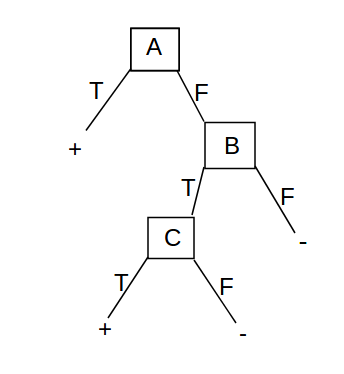
\includegraphics[width=.4\linewidth]{1b}
          }
    \end{minipage}
\item [c)]$[A \land B] \lor [C \land D]$
	\begin{minipage}[t]{\linewidth}
          \raggedright
          \adjustbox{valign=t}{
            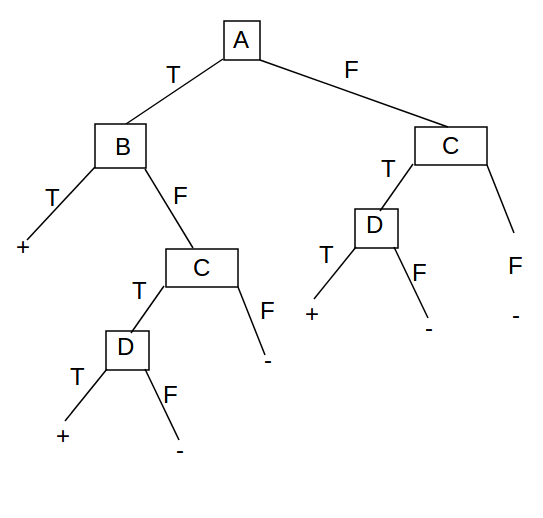
\includegraphics[width=.4\linewidth]{1c}
          }
    \end{minipage}
\end{enumerate}

\paragraph{2)}
Разгледайте следното множество от обучаващи примери: (T – истина; F – лъжа)

\begin{center}
  \begin{tabular}{ | c | c | c | c |}
    \hline
    Пример & Класификация & $A_1$ & $A_2$ \\ \hline
    1 & + & T & T \\ \hline
    2 & + & T & T \\ \hline
    3 & - & T & F \\ \hline
    4 & + & F & F \\ \hline
    5 & - & F & T \\ \hline
    6 & - & F & T \\ \hline
    \hline
  \end{tabular}
\end{center}

\begin{enumerate}
\item [a)]
Каква е ентропията на това множество от обучаващи примери по отношение
за целевата класификация?
\paragraph{Решение}
Ентропията се дефинира по следния начин:
\begin{gather}
	Entropy(S) = - \sum_{i=1}^c p_i \cdot \log_2 p_i
\end{gather}
В примерите имаме само два класа като три от примерите са положителни и три са отрицантелни
\begin{gather}
	Entropy(S) = - p_+ \cdot log_2 p_+ - p_- \cdot log_2 p_-
\end{gather}
\begin{gather}
	Entropy(S) = - 0.5 \cdot (-1) - 0.5 \cdot (-1) = 1
\end{gather}

\item [b)]
Каква е информационната печалба на атрибута $A_2$ по отношение на тези
примери?
\paragraph{Решение}
Информационната печалба се дефинира по следния начин:
\begin{gather}
	Gain(S, A) = Entropy(S) - \sum_{v \in Стойности(А)} \frac{\mathopen|S_v\mathclose|}{\mathopen|S\mathclose|} \cdot Entropy(S_v)
\end{gather}
Следователно за атрибута $A_2$ получаваме:
\begin{gather}
	Gain(S, A_2) = Entropy(S) - \sum_{v \in \{T, F\}} \frac{\mathopen|S_v\mathclose|}{\mathopen|S\mathclose|} \cdot Entropy(S_v)
\end{gather}
\begin{gather}
	Gain(S, A_2) = 1 - 
	\frac{\mathopen|S_T\mathclose|}
		{\mathopen|S\mathclose|} Entropy(S_T) - 				\frac{\mathopen|S_F\mathclose|}{\mathopen|S\mathclose|} \cdot Entropy(S_F)
\end{gather}
В $S_T$ попадат четири примера като два са положителни и два са отрицателни. В $S_F$ попадат два примера като един е положителен и един е отрицателен. По този начин получаваме:
\begin{gather}
	Entropy(S_T) = 1
\end{gather}
\begin{gather}
	Entropy(S_F) = 1
\end{gather}
\begin{gather}
	\Rightarrow
	Gain(S, A_2) = 1 - \frac{4}{6} \cdot 1 - \frac{2}{6}\cdot 1 = 
		1 - 1 = 0
\end{gather}
\end{enumerate}

\paragraph{3)}
\begin{enumerate}
\item [a)]
Начертайте класификационното дърво, което ще бъде научено от ID3
алгоритъма след четири обучаващи примера на понятието \textit{Харесва}, зададени
в Таблица 1 от лекция 1:
\begin{center}
  \begin{tabular}{ | c | c | c | c | c | c | c | c |}
    \hline
    Пример & Небе & Въздух & Влажност & Вятър & Вода & Прогноза & Харесва \\ \hline
    1 & Слънце & Топъл & Нормална & Силен & Топла & Същото & Да \\ \hline
    2 & Слънце & Топъл & Висока & Силен & Топла & Същото & Да \\ \hline
    3 & Дъжд & Студен & Висока & Силен & Топла & Промяна & Не \\ \hline
    4 & Слънце & Топъл & Висока & Силен & Студена & Промяна & Да \\
    \hline
  \end{tabular}
\end{center}
\paragraph{Решение}
Нека началното множество да се казва $S$. Нека положителните примери са тези дни, които човекът харесва, а отрицателните да са тези, който човекът не харесва. В $S$ има три положителни и един отрицателен пример като получаваме следната стойност за ентропията:
\begin{gather}
	Entropy(S) = - \frac{1}{4} \cdot \log_2 \frac{1}{4} - \frac{3}{4} \cdot \log_2 \frac{3}{4} = 0.5 + 0.311 = 0.811
\end{gather}
Така получаваме следните стойности за информационната печалба:
\begin{multline}
	Gain(S, \textup{ Небе}) = Entropy(S) - \frac{S_{\textup{слънце}}}{S} \cdot Entropy(S_{\textup{слънце}}) - \\ - \frac{S_{\textup{дъжд}}}{S} \cdot Entropy(S_{\textup{дъжд}})
\end{multline}
\begin{gather}
	\Rightarrow
	Gain(S, \textup{ Небе}) = 0.811 - \frac{3}{4} \cdot 0 - \frac{1}{4} \cdot 0 = 0.811
\end{gather}
Информационната печалба при разделяне по атрибута Небе е максимална, защото когато разделим по стойностите на Небе имаме множества, в които има само положителни или само отрицателни примери. Това означава, ентропиите на съответните множества ще са 0 и следователно информационната печалба ще е максимална - а именно равна на $Entropy(S)$. Това означава, че няма нужда да пресмятаме информационната печалба при разделяне по другите атрибути, защото тя ще е по-малка или равна на получената при разделяне по атрибута Небе. \\\\
Получава се следното класификационно дърво:\\\\
\begin{minipage}[t]{\linewidth}
          \raggedright
          \adjustbox{valign=t}{
            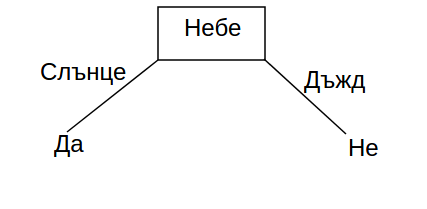
\includegraphics[width=.4\linewidth]{3a}
          }
\end{minipage}
\item [b)]
Добавете новия пример:
\begin{center}
  \begin{tabular}{ | c | c | c | c | c | c | c | c |}
    \hline
    Пример & Небе & Въздух & Влажност & Вятър & Вода & Прогноза & Харесва \\ \hline
    5 & Слънце & Топъл & Нормална & Слаб & Топла & Същото & Не \\
    \hline
  \end{tabular}
\end{center}
Постройте ново дърво и укажете стойността на информационната печалба за
всеки кандидат атрибут при всяка стъпка от построяването на дървото.
\paragraph{Решение}
С добавянето на новия пример получаваме и нова стойност за ентропията за множеството S:
\begin{gather}
	Entropy(S) = - \frac{2}{5} \cdot \log_2 \frac{2}{5} - \frac{3}{5} \cdot \log_2 \frac{3}{5} = 0.529 + 0.442 = 0.971
\end{gather}
Така получаваме и новата стойност за информационната печалба при разбиване по атрибута Небе:
\begin{multline}
	Gain(S, \textup{ Небе}) = Entropy(S) - \frac{S_{\textup{слънце}}}{S} \cdot Entropy(S_{\textup{слънце}}) - \\ - \frac{S_{\textup{дъжд}}}{S} \cdot Entropy(S_{\textup{дъжд}})
\end{multline}
За четири от петте примера имаме, че атрибута Небе е Слънце като три от тези четири имат стойност Да на атрибута Харесва и само един има стойност Не. За един от петте примера имаме, че атрибута Небе приема стойност Дъжд и когато имаме само един пример в това множество ентропията е 0. Когато разбием $S$ по атрибута Небе получаваме следните ентропии:
\begin{gather}
	Entropy(S_{\textup{слънце}}) = - \frac{1}{4} \cdot \log_2 \frac{1}{4} - \frac{3}{4} \cdot \log_2 \frac{3}{4} =  0.811
\end{gather}
\begin{gather}
	Entropy(S_{\textup{дъжд}}) = 0
\end{gather}
\begin{gather}
	\Rightarrow
	Gain(S, \textup{ Небе}) = 0.971 - \frac{4}{5} \cdot 0.811 - \frac{1}{5} \cdot 0 = 0.322
\end{gather}
Когато разбиваме по атрибута Въздух, получаваме същото разбиване на подмножества както при атрибута Небе:
\begin{gather}
	S_{\textup{слънце}} = S_{\textup{топъл}}
\end{gather}
\begin{gather}
	S_{\textup{дъжд}} = S_{\textup{студен}}
\end{gather}
Това означава, че ентропиите на подмножествата са равни и съответно и стойността на информационната печалба при разбиване по атрибута Въздух е същата като тази при разбиване по атрибута Небе:
\begin{gather}
	Gain(S, \textup{ Въздух}) = Gain(S, \textup{ Небе})
\end{gather}
За информационната печалба при разбиване по атрибута Влажност получаваме:
\begin{multline}
	Gain(S, \textup{ Влажност}) = Entropy(S) - \frac{S_{\textup{нормална}}}{S} \cdot Entropy(S_{\textup{нормална}}) - \\ - \frac{S_{\textup{висока}}}{S} \cdot Entropy(S_{\textup{висока}})
\end{multline}
В $S_{нормална}$ имаме два примера като единия е положителен, а другият отрицателен.
\begin{gather}
	Entropy(S_{\textup{нормална}}) = 1
\end{gather}
В $S_{висока}$ имаме три примера като два са положителни, а другият отрицателен.
\begin{gather}
	Entropy(S_{\textup{висока}}) = - \frac{2}{3} \cdot log_2 \frac{2}{3} - \frac{1}{3} \cdot log_2 \frac{1}{3} = 0.39 + 0.53 = 0.92
\end{gather}
\begin{gather}
	\Rightarrow
	Gain(S, \textup{ Влажност}) = 0.971 - \frac{2}{5} \cdot 1 - \frac{3}{5} \cdot 0.92 = 0.019
\end{gather}
Като следваме логиката за пресмятане от по-горе получаваме следната стойност за информационната печалба при разбиване по атрибута Вятър:
\begin{multline}
	Gain(S, \textup{ Вятър}) = Entropy(S) - \frac{S_{\textup{силен}}}{S} \cdot Entropy(S_{\textup{силен}}) \\ - \frac{S_{\textup{слаб}}}{S} \cdot Entropy(S_{\textup{слаб}})
\end{multline}
\begin{gather}
	Entropy(S_{\textup{силен}}) = - \frac{1}{4} \cdot \log_2 \frac{1}{4} - \frac{3}{4} \cdot \log_2 \frac{3}{4} =  0.811
\end{gather}
\begin{gather}
	Entropy(S_{\textup{слаб}}) = 0
\end{gather}
\begin{gather}
	\Rightarrow
	Gain(S, \textup{ Вятър}) = 0.971 - \frac{4}{5} \cdot 0.811 - \frac{1}{5} \cdot 0 = 0.322
\end{gather}
Забелязва се, че когато разбиваме по този атрибут получаваме същата информационна печалба както при разбиването при атрибутите Небе и Въздух, въпреки че подмножествата са различни. Това се получава, защото всъщност състава на множествата е еднакъв. Т.е. и при трите атрибута се разбива на две множества като едното множество има само един елемент, а другото множество има четири като три от четирите примера са от една категория, а последния е от различна. Това означава, че ентропиите на множествата ще са еднакви и съответно и информационната печалба ще е същата.
За информационната печалба при разбиване по атрибута Вода получаваме:
\begin{multline}
	Gain(S, \textup{ Вода}) = Entropy(S) - \frac{S_{\textup{топла}}}{S} \cdot Entropy(S_{\textup{топла}}) \\ - \frac{S_{\textup{студена}}}{S} \cdot Entropy(S_{\textup{студена}})
\end{multline}
\begin{gather}
	Entropy(S_{\textup{студена}}) = 0
\end{gather}
\begin{gather}
	Entropy(S_{\textup{топла}}) = - \frac{2}{4} \cdot \log_2 \frac{2}{4} - \frac{2}{4} \cdot \log_2 \frac{2}{4} =  1
\end{gather}
\begin{gather}
	\Rightarrow
	Gain(S, \textup{ Вода}) = 0.971 - \frac{4}{5} \cdot 1 - \frac{1}{5} \cdot 0 = 0.171
\end{gather}
За информационната печалба при разбиване по атрибута Прогноза получаваме:
\begin{multline}
	Gain(S, \textup{ Прогноза}) = Entropy(S) - \frac{S_{\textup{същата}}}{S} \cdot Entropy(S_{\textup{същата}}) - \\ - \frac{S_{\textup{промяна}}}{S} \cdot Entropy(S_{\textup{промяна}})
\end{multline}
\begin{gather}
	Entropy(S_{\textup{същата}}) = - \frac{2}{3} \cdot \log_2 \frac{2}{3} - \frac{1}{3} \cdot \log_2 \frac{1}{3} =   0.92
\end{gather}
\begin{gather}
	Entropy(S_{\textup{промяна}}) = - \frac{1}{2} \cdot \log_2 \frac{1}{2} - \frac{1}{2} \cdot \log_2 \frac{1}{2} =  1
\end{gather}
\begin{gather}
	\Rightarrow
	Gain(S, \textup{ Прогноза}) = 0.971 - \frac{3}{5} \cdot 0.92 - \frac{2}{5} \cdot 1 = 0.019
\end{gather}
От получените стойности за информационната печалба имаме най-висока стойност от 0.322, която се постига при разбиването на един от атрибутите Небе, Въздух или Вятър. Нека си изберем и да разбием множеството по атрибута Небе. Така получаваме две множества: $S_1$, в което има примери 1, 2, 4 и 5 и $S_2$, в което има само пример 4.
За множеството $S_2$ имаме ентропия 0, защото там има само един пример, затова там няма нужда да разбиваме повече, а можем да заключим, че ако стойността на небе е Дъжд, то човекът не харесва този ден. \\\\
Нека сега да видим по кой атрибут е най-добре да разбием множеството $S_1$. За целта отново трябва да изчислим информационните печалби. Първо нека сметнем стойността на ентропията за множеството $S_1$:
\begin{gather}
	Entropy(S_1) = - \frac{3}{4} \cdot \log_2 \frac{3}{4} - \frac{1}{4} \cdot \log_2 \frac{1}{4} =  0.811
\end{gather}
Ако разбием по атрибута Въздух няма да получим никаква печалба, защото всички примери от множеството $S_1$ имат стойност за атрибута Топъл.
\begin{gather}
	\Rightarrow
	Gain(S_1, \textup{ Въздух}) = 0
\end{gather}
За информационната печалба при разбиване по атрибута Влажност имаме:
\begin{multline}
	Gain(S_1, \textup{ Влажност}) = \\ Entropy(S_1) - \frac{S_{\textup{1, нормална}}}{S_1} \cdot Entropy(S_{\textup{1, нормална}}) -  \\ - \frac{S_{\textup{1, висока}}}{S_1} \cdot Entropy(S_{\textup{1, висока}})
\end{multline}
\begin{gather}
	Entropy(S_{\textup{1, нормална}}) = - \frac{1}{2} \cdot \log_2 \frac{1}{2} - \frac{1}{2} \cdot \log_2 \frac{1}{2} = 1
\end{gather}
\begin{gather}
	Entropy(S_{\textup{1, висока}}) = 0
\end{gather}
\begin{gather}
	\Rightarrow
	Gain(S, \textup{ Влажност}) = 0.811 - \frac{2}{4} \cdot 1 - \frac{2}{4} \cdot 0 = 0.311
\end{gather}
За информационната печалба при разбиване по атрибута Вятър имаме:
\begin{multline}
	Gain(S_1, \textup{ Вятър}) = \\ Entropy(S_1) - \frac{S_{\textup{1, силен}}}{S_1} \cdot Entropy(S_{\textup{1, силен}}) -  \\ - \frac{S_{\textup{1, слаб}}}{S_1} \cdot Entropy(S_{\textup{1, слаб}})
\end{multline}
\begin{gather}
	Entropy(S_{\textup{1, силен}}) = 0
\end{gather}
\begin{gather}
	Entropy(S_{\textup{1, слаб}}) = 0
\end{gather}
\begin{gather}
	\Rightarrow
	Gain(S, \textup{ Вятър}) = 0.811
\end{gather}
При разбиване по атрибута Вятър получаваме две подмножества с като в едното са само положителни, а в другото само отрицателни. Това означава, че ентропиите на съответните множества са 0, което от своя страна означава, че имаме максимална стойност на информационната печалба. Няма смисъл да разглеждаме информационната печалба за другите атрибути, защото тя няма как да е по-голяма от тази.
Класификационното дърво има следния вид:\\\\
\begin{minipage}[t]{\linewidth}
          \raggedright
          \adjustbox{valign=t}{
            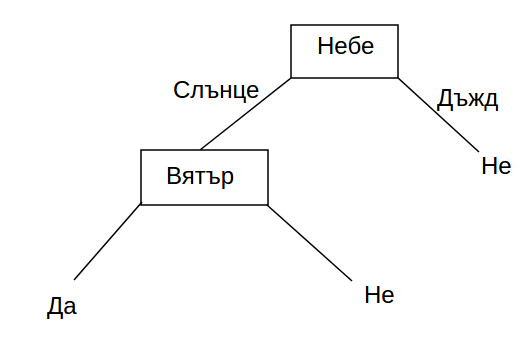
\includegraphics[width=.4\linewidth]{3b}
          }
\end{minipage}
\end{enumerate}
\end{document}